\documentclass[11pt, a4paper]{report}
\usepackage{fontspec}
\setmainfont[Script=Greek]{GFS Artemisia}
\setmonofont{FreeMono}

\usepackage{polyglossia}
\setdefaultlanguage{greek}
\setotherlanguages{english}

\usepackage{geometry}
\geometry{margin=3cm}

\usepackage{minted2}
\usepackage{graphicx}

\begin{document}
% header section
\author{Πλαστήρας Πέτρος}
\title{Εργασία \#2 - Μέρος B}
\date{\today}
\maketitle

\section{Άσκηση 1}
Σχεδιάστε ένα συνδυαστικό λογικό κύκλωμα σε VHDL το οποίο υλοποιεί τις ακόλουθες λογικές και αριθμητικές πράξεις (ALU) ανάλογα με τις τιμές των σημάτων $S_1, S_0, C_{in}$.

\begin{center}
	\begin{tabular}{|c|c|c|c|}
		\hline
		$S_1$ & $S_0$ & $C_{in}$ & Πράξη                           \\
		\hline
		0     & 0     & x        & $Y = A - B + C_{in}$            \\
		0     & 1     & x        & $Y = Shift Right Arithmetic(A)$ \\
		1     & 0     & 0        & $Y = Shift Logical Right(B)$    \\
		1     & 0     & 1        & $Y = Shift Logical Left(A)$     \\
		1     & 1     & x        & $Y = \overline{A \cdot B}$      \\
		\hline
	\end{tabular}
\end{center}

Σας δίνεται ο ορισμός της οντότητας:
\inputminted[firstline=5, lastline=14]{vhdl}{./code/part-2/alu-1/alu.vhdl}

Για την υλοποίηση της αρχιτεκτονικής της οντότητας, αφού το κύκλωμα είναι συνδυαστικό αρκεί να χρησιμοποιήσουμε μια αρχιτεκτονική μορφής Dataflow. Συγκεκριμένα, θα συνδυάσουμε τα σήματα $S_0$ και $S_1$ σε ένα σήμα
\mintinline{vhdl}{std_logic_vector} των 2 bit, το οποίο ονομάζουμε $S$.
Στην συνέχεια με την χρήση μιας δομής \mintinline{vhdl}{with S select} θα μπορούμε να επιλέξουμε το αποτέλεσμα του κυκλώματός μας για τις διάφορες τιμές του $S$.

Τώρα για τον υπολογισμό των αποτελεσμάτων, θα χρησιμοποιοίσουμε τα παρακάτω:
\begin{enumerate}
	\item Αρχικά για την περίπτωση που $S = 00$, θα χρησιμοποιήσουμε τον τύπο \mintinline{vhdl}{signed} από το πακέτα \mintinline{vhdl}{numeric_std}.
	      Για να γίνει αυτό πρέπει να μετατρέψουμε το $A$, το $B$ και το $C_{in}$ σε \mintinline{vhdl}{signed}.
	      Το $C$ χρειάζεται αρχικά να μετατρεπεί από \mintinline{vhdl}{std_logic} σε \mintinline{vhdl}{std_logic_vector} των 8 bit.
	      Ύστερα μπορούμε απλά να αφαιρέσουμε το $A$ και το $B$ να προσθέσουμε το $C$ και να μετατρέψουμε το αποτέλεσμα πίσω σε \mintinline{vhdl}{std_logic_vector}.
	\item Στην περίπτωση που $S = 01$ θα μετατρέψουμε το $Α$ σε \mintinline{vhdl}{signed} και στην συνέχεια θα χρησιμοποιήσουμε την συνάρτηση
	      \mintinline{vhdl}{shift_right} η οποία αν η είσοδός της είναι προσημασμένος, παραγματοποιεί αριθμητική ολίσθηση.
	\item Αν το $S = 10$ θα χρησιμοποιήσουμε ένα νέο εσωτερικό σήμα, το οποίο υλοποιεί την λογική της ολίσθησης ανάλογα με την τιμή του $C_{in}$.
	      Αν είναι 0, κάνει δεξιά ολίσθηση το σήμα $B$ ενώ αν είναι ένα κάνει αριστερή ολίσθηση το σήμα $Α$. Το παραπάνω υλοποιείται επίσης με την χρήση μιας δομής \mintinline{vhdl}{with Cin select}.
	\item Τέλος, αν $S = 11$ μπορούμε άμεσα με την χρήση του τελεστή \mintinline{vhdl}{nand} να υλοποιήσουμε την πράξη $\overline{A \cdot B}$.
\end{enumerate}

Σύμφωνα μα τα παραπάνω προκύπτει ο παρακάτω κώδικας για την οντότητα $ALU$:
\inputminted[breaklines, linenos]{vhdl}{./code/part-2/alu-1/alu.vhdl}

Για το αρχείο της προσομοίωσης απλά ελέγχουμε κάποιες ενδεικτικές περιπτώσεις, με θετικούς και αρνητικούς αριθμούς:
\inputminted[breaklines, linenos]{vhdl}{./code/part-2/alu-1/alu_tb.vhdl}

\newpage
 
Αφού έχουμε κάνει τα παραπάνω μπορούμε να κάνουμε RTL ανάλυση της οντότητάς μας. Το αποτέλεσμα φαίνεται παρακάτω:
\begin{center}
	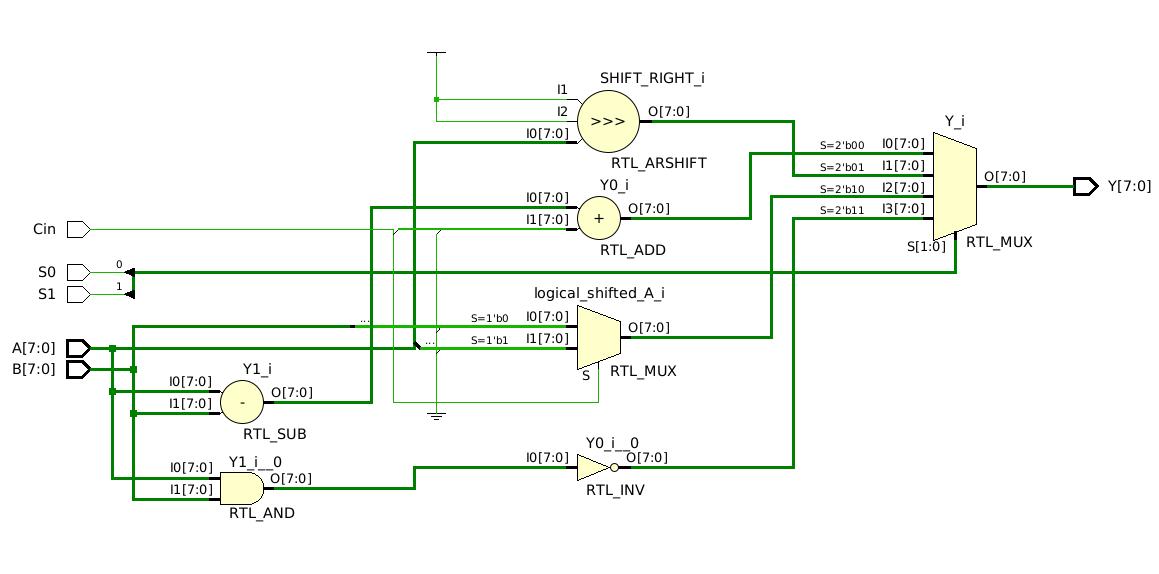
\includegraphics[width=\textwidth]{./images/alu-1/RLT_ALU.png}
\end{center}

Τρέχοντας την προσομοίωση, προκύπτει η παρακάτω κυματομορφή:
\begin{center}
	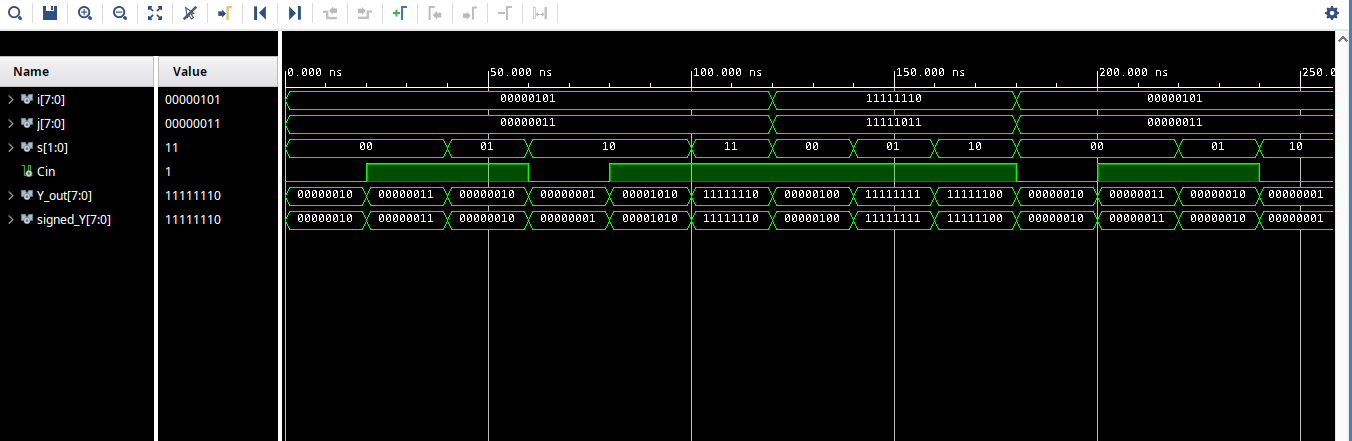
\includegraphics[width=\textwidth]{./images/alu-1/Behavioral_Sim_Fixed.png}
\end{center}

Στην συνέχεια μπορούμε να κάνουμε σύνθεση, η οποία δημιουργεί το παρακάτω schematic:
\begin{center}
  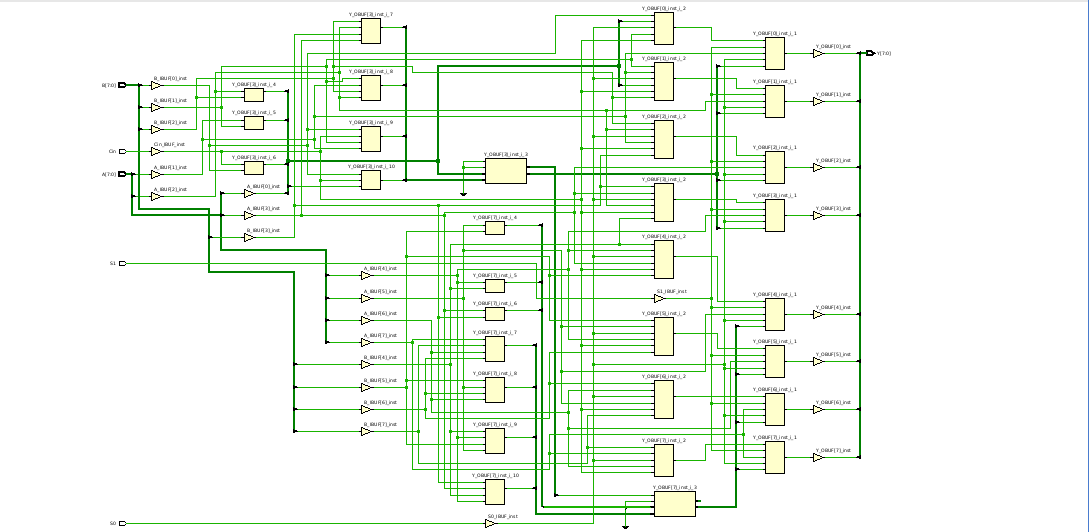
\includegraphics[width=\textwidth]{./images/alu-1/Synth_Schematic.png}
\end{center}

Μετά απο αυτό μπορεί να γίνει και Post-Synthesis Timing Simulation, η οποία δημιουργεί την παρακάτω κυματομορφή:
\begin{center}
  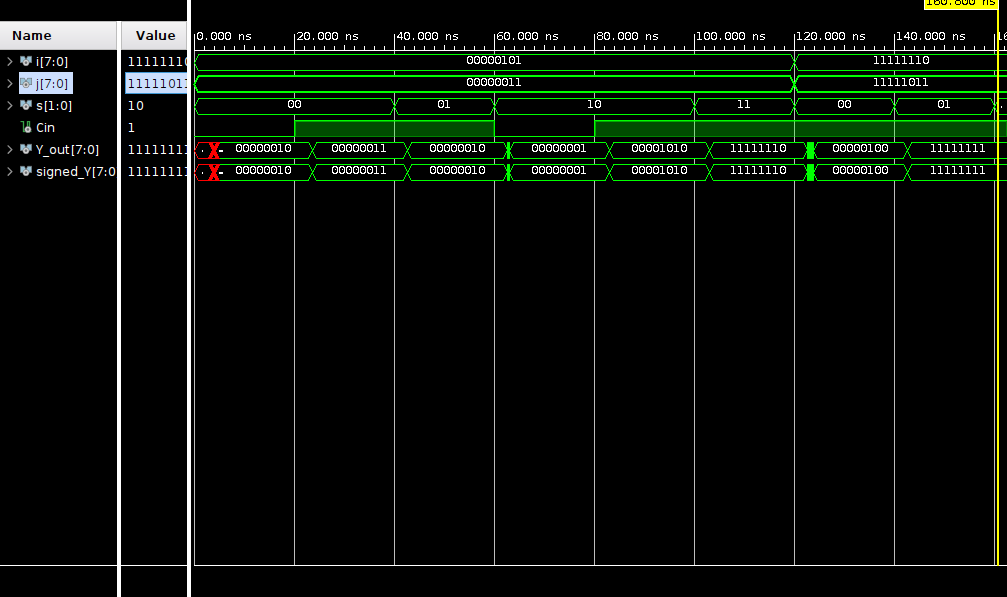
\includegraphics[width=\textwidth]{./images/alu-1/PST_Fixed.png}
\end{center}

Μπορούμε να βρούμε τους πόρους που χρησιμοποιεί η υλοποίησή μας, χρησιμοποιούμε το Report Utilization το οποίο παράγει τον παρακάτω πίνακα:
\begin{center}
  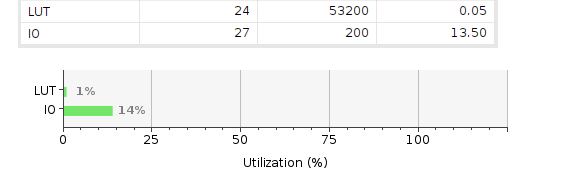
\includegraphics[width=\textwidth]{./images/alu-1/Utilization.png}
\end{center}

Αυτό σημαίνει ότι χρησιμοποιούμε 24 lookup tables και 27 IO buffers για ενίσχυση του εισερχόμενου ή εξερχόμενου σήματος.

Τέλος, μπορούμε να κάνουμε Report Timings και πηγαίνοντας στο Summary να δούμε τα παρακάτω σχετικά με τις καθυστερήσεις διάδοσης και μόλυνσης αντίστοιχα:
\begin{center}
  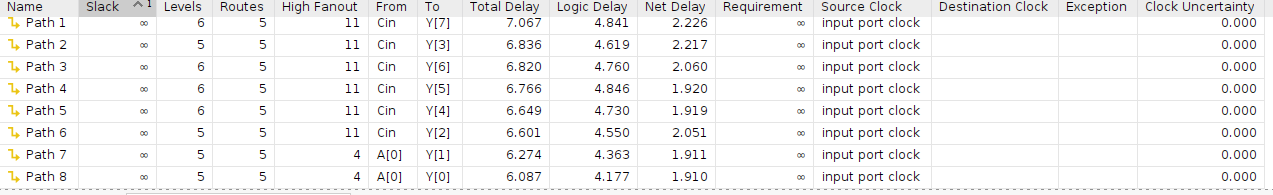
\includegraphics[width=\textwidth]{./images/alu-1/Setup_Time_Summury.png}
  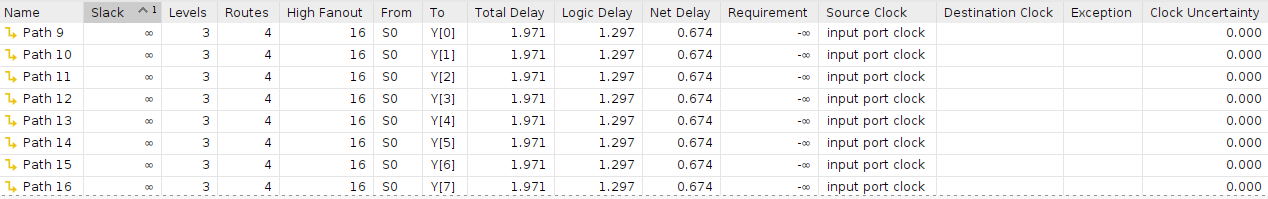
\includegraphics[width=\textwidth]{./images/alu-1/Hold_Time_Summury.png}
\end{center}

Από το παραπάνω, κάνοντας διπλό κλικ στο πιο αργό και στο πιο γρήγορο μονοπάτι αντίστοιχα, μπορούμε να τα δούμε πάνω στο σχεδιάγραμα:
\begin{center}
  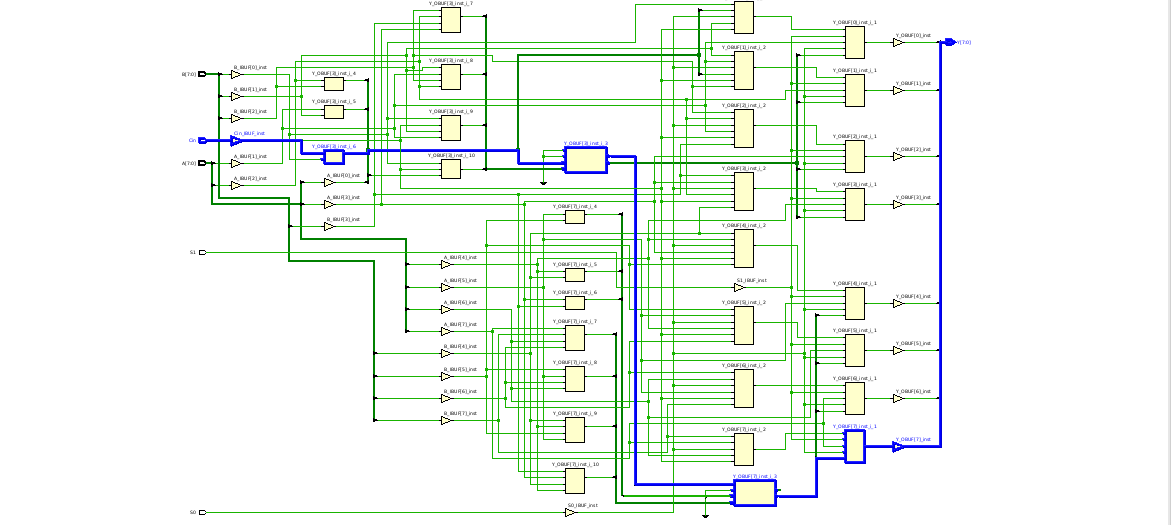
\includegraphics[width=\textwidth]{./images/alu-1/Slowest_Path.png}
  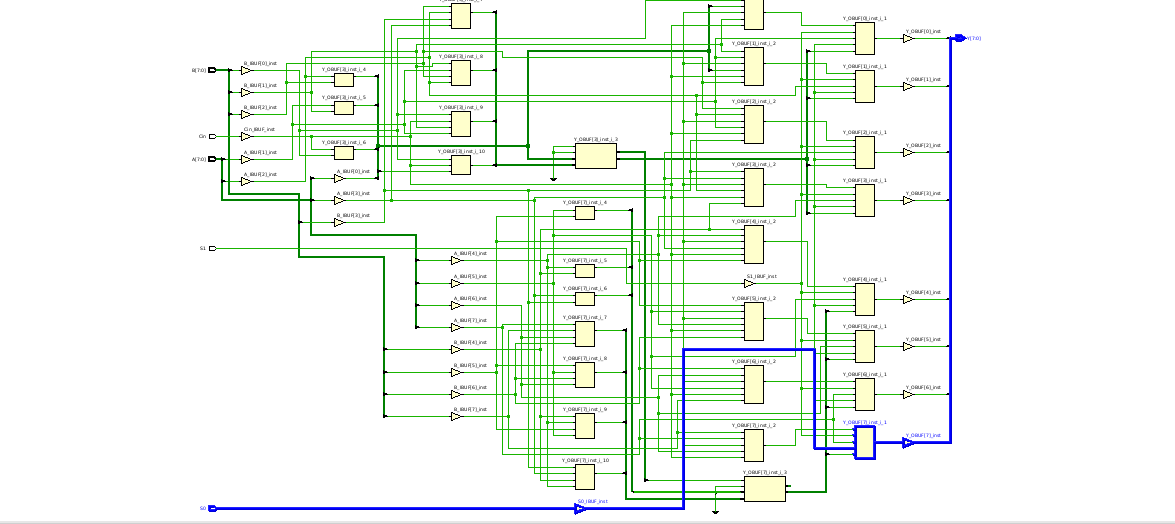
\includegraphics[width=\textwidth]{./images/alu-1/Fastest_Path.png}
\end{center}

\end{document}
